\subsection{Compass Implementation}
As the IMU was connected to one of the ZedBoard's Pmod connectors, it had the option of being controlled by either the Programmable Logic (PL) or the Programmable Software (PS). The IMU's magnetometer data was be used to rotate the rangefinder data according to a compass direction by offsetting the rangefinder's step value. Since the step value was set in the PS, all of the IMU's implementation has the ability to be done in the PS, which is a simpler and quicker solution than taking advantage of the PS-PL communication setup from Section \ref{ssec:ps_pl}. Another motivation for using the PS is that the IMU data processing involves complex trigonometry, which is simpler done in the PS than by using a CORDIC function in the PL.
\par
As such, the Zynq7 Processing System was re-customized to provide this capability.

\subsubsection{Re-Customizing the Zynq7 Processing System}
The Zynq7 Processing System is easily re-customizable, as discussed in Section \ref{zynq7processingsystem}. SPI functionality was added in the processing system's customization window under I/O Peripherals in the MIO Configuration tab. The SPI pins were routed to Extended MIO (EMIO) so that the ZedBoard's PL Pmod was controlled from the PS. Since both SPI0 and SPI1 have EMIO functionality, SPI0 was chosen over SPI1. This process is shown in Figure \ref{enabling_spi0}.

\begin{figure}[H]
	\centerline{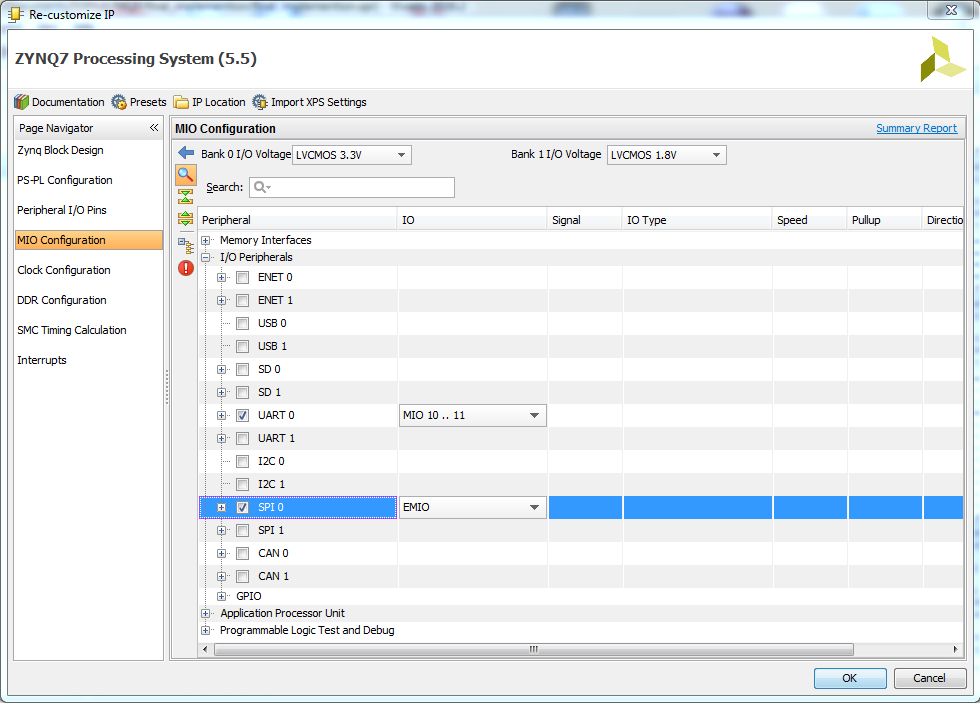
\includegraphics[width=1\textwidth]{enabling_spi0.png}}
	\caption{Re-Customizing the Zynq7 Processing System to Add SPI}
	\label{enabling_spi0}
\end{figure}

\par
EMIO functionality allows for pins normally connected to the Zynq7 processor's programmable logic to be connected to the processor's programmable software instead. In other words, EMIO peripherals allow for the user to control physical pins using C code running on the Zynq7 dual ARM processors rather than in Verilog-defined hardware. By creating an EMIO SPI peripheral, it was possible to route the physical connection of the interface to any pin on the ZedBoard that is accessible by programmable logic. In the case of this specific implementation, the EMIO SPI peripheral was routed to one of the ZedBoard's Pmod ports, allowing for the MIO Pmod port to remain unused and open for I$^2$C and UART peripheral communications.






